\chapter{Fisiologi Ginjal dan Osmoregulasi}\label{ch:b3:renal-osmoregulation}

Ginjal Anda menapis seratus delapan puluh liter plasma tiap hari ---
seluruh volume darah Anda tiap setengah jam --- lalu mengembalikan semuanya
kecuali satu setengah liter, sesudah mengeluarkan ureanya, menyesuaikan garam,
asam, dan airnya sampai dalam satu persen dari yang diperlukan tubuhnya, serta
menahan tiap gram glukosanya. Seekor tikus kanguru di gurun tidak pernah minum
sama sekali: ia hidup dari air yang dibuat metabolismenya dari biji kering lalu
mengekskresikan kemih lima kali lebih pekat daripada air laut. Seekor ikan laut
minum terus-menerus lalu memompa garamnya keluar lewat insangnya; seekor ikan
air tawar tidak pernah minum lalu memompa garam masuk. Masalah yang
diselesaikan mereka semua sama: menahan susunan cairan di sekeliling
selnya tetap sementara makan, minum, dan bernapas
mengganggunya, serta membuang nitrogen tanpa membuang terlalu banyak
air. Bab ini memperlakukan ginjal mamalia sebagai contoh yang digarap
--- penapisan, aritmetika bersihan, muslihat arus balik
yang memekatkan kemih, dan hormon yang menetapkan
tombolnya --- lalu keragaman penyelesaian di antara hewan.

\section{Masalahnya}

\begin{definition}[Osmoregulasi]\label{def:b3:renal-osmoregulation:problem}
\index{osmolaritas}\index{tekanan osmosis}\index{cairan luar sel}%
\index{osmokonformer}\index{osmoregulator}
\emph{Osmolaritas} sebuah larutan adalah kepekatan total partikel
terlarutnya (dalam osmol tiap liter); ia menetapkan \emph{tekanan
osmosis}, $\Pi = cRT$ bagi larutan encer, yang mendorong air melintasi
selaput apa pun yang melewatkan air tetapi bukan zat terlarutnya. Cairan tubuh seekor mamalia
duduk pada sekitar \qty{300}{mOsm/L} --- \qty{40}{\%} massa tubuhnya di dalam
selnya, \qty{20}{\%} di luarnya, yakni \emph{cairan luar sel} yang
seperempatnya plasma --- dan selnya mengembang atau menyusut dalam hitungan detik bila
luarnya berubah, sebab selaputnya melewatkan air dengan bebas. Sebuah
\emph{osmokonformer} (kebanyakan hewan laut tak bertulang belakang, hiu) menjaga
cairannya pada osmolaritas lautnya lalu mengatur susunannya saja;
sebuah \emph{osmoregulator} (vertebrata, serangga,
hewan air tawar) menahan osmolaritasnya tetap terhadap
lingkungannya, yang berongkos tenaga sebanding dengan landaiannya.
Tugas keduanya, yang tergandeng pada yang pertama, adalah membuang nitrogen dari
perombakan protein: sebagai \emph{amonia} ke dalam air yang berlimpah (ikan), sebagai
\emph{urea}, yang larut dan tidak beracun tetapi memerlukan air untuk mengusungnya
(mamalia), atau sebagai \emph{asam urat}, yakni sebuah pasta yang diekskresikan nyaris kering (burung,
reptil, serangga).
\end{definition}

\section{Nefron dan penapisan}

\begin{definition}[Nefron]\label{def:b3:renal-osmoregulation:nephron}
\index{nefron}\index{glomerulus}\index{tubulus proksimal}%
\index{lengkung Henle}\index{saluran pengumpul}
Tiap ginjal manusia memuat sekitar sejuta \emph{nefron}. Darah memasuki
sebuah \emph{glomerulus}, yakni seberkas kapiler di dalam kapsul Bowman, yang
dindingnya --- endotelium bertingkap, selaput dasar, serta
diafragma celah di antara kaki podositnya --- melewatkan air dan tiap zat terlarut
di bawah sekitar \qty{60}{kDa} tetapi menahan protein dan selnya. Tapisannya
mengalir menembus \emph{tubulus proksimal}, yang menyerap kembali dua
pertiga air dan garamnya serta seluruh glukosa dan asam aminonya; turun
dan naik \emph{lengkung Henle}, yang menjangkau ke dalam medulanya lalu
membangun landaian kepekatan bagian berikutnya; menembus
\emph{tubulus distal}, tempat garamnya disesuaikan; lalu ke dalam
\emph{saluran pengumpul}, tempat kandungan air akhirnya ditetapkan
vasopresin ketika salurannya melewati medulanya ke pialanya. Darah
yang meninggalkan glomerulusnya memasuki sebuah petak kapiler kedua di sekeliling
tubulusnya, yang mengambil apa yang diserapnya kembali.
\end{definition}

\begin{omfigure}
\begin{tikzpicture}[every node/.style={font=\scriptsize}, >=stealth]
  % cortex/medulla background
  \fill[omDef!6] (-0.5,0) rectangle (11.5,3.6); \fill[omProp!8] (-0.5,-3.4) rectangle (11.5,0);
  \node[right, gray] at (-0.4,3.4) {korteks}; \node[right, gray] at (-0.4,-3.2) {medula};
  % glomerulus
  \draw[thick, omThm, fill=omThm!20] (0.8,2.6) circle (0.55); \node[below, align=center] at (0.25,2.0) {glomerulus:\\penapisan,\\\qty{180}{L/d}};
  % proximal tubule
  \draw[very thick, omDef] (1.35,2.6) .. controls (2.2,3.3) and (2.8,2.0) .. (3.2,2.6) .. controls (3.5,3.1) and (3.9,2.2) .. (4.2,2.6);
  \node[below, align=center] at (2.65,2.05) {tubulus proksimal:\\\qty{67}{\%} Na$^{+}$ dan air,\\semua glukosa, asam amino,\\HCO$_3^-$};
  % loop of Henle
  \draw[very thick, omDef] (4.2,2.6) -- (4.2,-2.8) arc[start angle=180, end angle=360, radius=0.4] -- (5.0,2.6);
  \node[left, align=right] at (4.1,-1.0) {cabang turun:\\air pergi};
  \node[right, align=left] at (5.1,-1.6) {cabang naik:\\NaCl dipompa keluar,\\tanpa air};
  \node[right, align=left, omProp!80!black] at (5.1,-0.2) {\qty{25}{\%} Na$^{+}$};
  % distal tubule
  \draw[very thick, omDef] (5.0,2.6) .. controls (5.4,3.2) and (6.0,2.0) .. (6.4,2.6) .. controls (6.8,3.1) .. (7.2,2.6);
  \node[above, align=center] at (6.0,3.1) {tubulus distal: Na$^{+}$ (aldosteron),\\sekresi Ca$^{2+}$, K$^{+}$};
  % collecting duct
  \draw[very thick, omMeth!70!black] (7.2,2.6) -- (7.8,2.6) -- (7.8,-3.2);
  \node[right, align=left] at (7.9,-1.2) {saluran pengumpul:\\air (vasopresin,\\akuaporin-2),\\urea, H$^{+}$;\\\qty{1.5}{L/d} keluar};
  \draw[->, thick, omMeth!70!black] (7.8,-3.2) -- (7.8,-3.6);
  % osmolarity scale on the right
  \foreach \y/\c in {2.6/300, 0.0/600, -1.4/900, -2.8/1200} { \node[left, omProp!80!black, font=\tiny] at (11.4,\y) {\c\ mOsm}; }
  \draw[->, omProp!80!black] (11.4,2.9) -- (11.4,-3.1); \node[above, omProp!80!black, font=\tiny, align=center] at (11.4,3.0) {osmolaritas\\interstisium};
\end{tikzpicture}

{\small Sebuah \omterm{def:b3:renal-osmoregulation:nephron}{nefron} yang dibentangkan. Penapisan di dalam korteksnya; penyerapan
kembali besar-besaran di dalam \omterm{def:b3:renal-osmoregulation:nephron}{tubulus proksimalnya}; \omterm{def:b3:renal-osmoregulation:nephron}{lengkung Henle} yang mencelup ke dalam medulanya,
tempat interstisiumnya bertambah asin seiring kedalamannya; \omterm{def:b3:renal-osmoregulation:nephron}{saluran pengumpulnya}
yang lewat kembali menembus landaian itu lalu menyerahkan airnya bila vasopresinnya
mengizinkan.}
\end{omfigure}

\begin{theorem}[Penapisan dan bersihan]\label{thm:b3:renal-osmoregulation:clearance}
\index{gaya Starling}\index{laju filtrasi glomerulus}%
\index{bersihan}\index{inulin}\index{kreatinin}
Tapisannya mengalir melintasi dinding \omterm{def:b3:renal-osmoregulation:nephron}{glomerulusnya} pada sebuah laju yang ditetapkan
\emph{\omterm{thm:b3:renal-osmoregulation:clearance}{gaya Starling}}: tekanan hidrostatis kapilernya
$P_{\text{KG}}$ mendorong cairannya keluar, tekanan hidrostatis di dalam ruang
Bowman $P_{\text{RB}}$ dan tekanan onkotik protein plasmanya
$\pi_{\text{KG}}$ menariknya kembali, dan
\[
\text{LFG} = K_{f}\,\bigl(P_{\text{KG}} - P_{\text{RB}} - \pi_{\text{KG}}\bigr)
\approx K_{f}\,(55 - 15 - 30)\ \unit{mmHg} = K_{f}\times \qty{10}{mmHg},
\]
yakni \emph{\omterm{thm:b3:renal-osmoregulation:clearance}{laju filtrasi glomerulus}}, sekitar \qty{125}{mL/min} pada seorang
dewasa. Bagi sembarang zat $x$ berkepekatan plasma $P_{x}$, kepekatan
kemih $U_{x}$, dan aliran kemih $V$, \emph{bersihan}-nya
\[
C_{x} = \frac{U_{x}\,V}{P_{x}}
\]
adalah volume plasma yang dibersihkan dari $x$ tiap satuan waktu. Bila $x$ ditapis
dengan bebas dan tidak diserap kembali maupun disekresikan (inulin, dan nyaris demikian
kreatinin), $C_{x} = \text{LFG}$; bila ia disingkirkan sepenuhnya dari
plasma yang melewati ginjalnya (para-aminohipurat pada dosis rendah), $C_{x}$
sama dengan aliran plasma ginjalnya; sebuah bersihan di bawah LFG berarti penyerapan
kembali neto, di atasnya berarti sekresi neto, dan muatan tapisan $\text{LFG}
\times P_{x}$ dikurangi ekskresinya $U_{x}V$ adalah jumlah yang diserap kembali.
\end{theorem}
\begin{proof}
Penapisannya adalah ultrapenapisan menembus sebuah dinding berliang: alirannya
sebanding dengan tekanan neto yang melintasinya, dan tekanan netonya adalah
tekanan hidrostatis ke luar dikurangi tekanan hidrostatis dan onkotik ke
dalam (Starling), dengan tekanan onkotik tapisannya
terabaikan sebab ia tidak memuat protein. Bersihannya: dalam satuan waktu,
ginjalnya mengekskresikan $U_{x}V$ dari $x$; volume plasma yang memuat jumlah
ini adalah $U_{x}V/P_{x}$. Bagi sebuah zat yang hanya ditapis, apa
yang diekskresikan adalah apa yang ditapis, $\text{LFG}\times P_{x} = U_{x}V$,
yang darinya $C_{x} = \text{LFG}$. Bagi zat yang dipetik seluruhnya, semua $x$ di dalam
plasma yang mengalir lewat, $\text{APG}\times P_{x}$, diekskresikan,
yang darinya $C_{x} = \text{APG}$. Neraca massanya memberikan jumlah yang diserap kembali.
\end{proof}

\begin{example}[Bersihan dalam angka]\label{ex:b3:renal-osmoregulation:numbers}
Inulin yang diinfuskan sampai aras plasma \qty{1}{mg/mL} muncul di dalam kemih pada
\qty{125}{mg/mL} dengan aliran \qty{1}{mL/min}: $C = 125\times 1/1 =
\qty{125}{mL/min}$, yakni LFG-nya, \qty{180}{L/d}. Para-aminohipurat
memberi \qty{650}{mL/min}, yakni aliran plasmanya; dengan hematokrit $0.45$,
aliran darah ginjalnya \qty{1.2}{L/min}, seperlima keluaran
jantungnya bagi \qty{0.5}{\%} massa tubuhnya, dan pecahan penapisannya
$125/650 = 0.19$. Urea: plasma \qty{5}{mmol/L}, kemih \qty{300}{mmol/L}
pada \qty{1}{mL/min} --- bersihan \qty{60}{mL/min}, yakni separuh LFG-nya, sehingga separuh
urea yang ditapis diserap kembali. Glukosa: bersihannya nol pada aras
plasma yang normal, dengan tiap molekul dari \qty{180}{g} yang ditapis tiap hari
dikembalikan. Kreatinin, yang dibuat otot pada laju tetap dan hanya
ditapis, menjadi ukuran LFG milik klinik: ketika LFG-nya terbelah dua,
kreatinin plasmanya berlipat dua, tanpa pengumpulan kemih apa pun.
\end{example}

\begin{method}[Mengukur fungsi ginjal]\label{met:b3:renal-osmoregulation:gfr}
\index{pengukuran LFG}
(1) Bagi sebuah nilai penelitian, infuskanlah inulin sampai sebuah aras plasma yang mantap,
kumpulkanlah kemih bertakar waktu, ukurlah keduanya, lalu hitunglah $UV/P$. (2) Di
klinik, ukurlah kreatinin plasmanya lalu taksirlah LFG-nya darinya
dengan sebuah rumus yang mengoreksi umur, jenis kelamin, dan ukuran tubuh; taksirannya
adalah yang dengannya tahapan penyakit ginjal menahun didefinisikan (sebuah LFG
di bawah \qty{60}{mL/min} selama tiga bulan). (3) Ujilah keterpilihan
tapisannya dengan mengukur albumin di dalam kemihnya --- biasanya di bawah
\qty{30}{mg/d}; lebih daripada itu berarti sebuah penghadang yang bocor, yakni tanda paling awal
kerusakan ginjal diabetes. (4) Ujilah kemampuan memekatkannya dengan
menahan air semalaman lalu mengukur \omterm{def:b3:renal-osmoregulation:problem}{osmolaritas} kemihnya, yang
mestinya melebihi \qty{800}{mOsm/L}; kegagalan memekatkan dengan LFG yang
normal menunjuk ke \omterm{def:b3:renal-osmoregulation:nephron}{saluran pengumpulnya} atau ke vasopresinnya.
\end{method}

\begin{omfigure}
\begin{tikzpicture}
\begin{axis}[
  width=0.68\linewidth, height=5.6cm,
  axis x line=bottom, axis y line=left,
  xmin=0, xmax=800, ymin=0, ymax=700,
  xlabel={glukosa plasma (mg/dL)}, ylabel={mg/min},
  xlabel style={font=\small, at={(axis description cs:0.5,-0.12)}, anchor=north}, ylabel style={font=\small},
  tick label style={font=\small}, xtick={0,100,200,300,400,600,800}, ytick={0,200,375,600},
  clip=false,
]
\addplot[very thick, omDef, domain=0:800, samples=2] {1.25*x};
\addplot[very thick, omMeth!70!black, domain=0:200, samples=2] {1.25*x};
\addplot[very thick, omMeth!70!black, smooth] coordinates {(200,250) (250,300) (300,340) (350,365) (400,375) (800,375)};
\addplot[very thick, omThm, domain=0:180, samples=2] {0};
\addplot[very thick, omThm, smooth] coordinates {(180,0) (250,12) (300,35) (350,72) (400,125) (800,625)};
\draw[dashed, gray] (axis cs:180,0) -- (axis cs:180,700); \node[font=\scriptsize, gray, anchor=north west] at (axis cs:185,560) {ambang};
\draw[dashed, gray] (axis cs:0,375) -- (axis cs:800,375);
\node[font=\scriptsize, omDef, anchor=south east] at (axis cs:480,620) {ditapis: LFG $\times$ P};
\node[font=\scriptsize, omMeth!70!black, anchor=south west, align=left] at (axis cs:660,395) {diserap kembali:\\$T_{m} = \qty{375}{mg/min}$};
\node[font=\scriptsize, omThm, anchor=north west] at (axis cs:520,300) {diekskresikan};
\end{axis}
\end{tikzpicture}

{\small Kurva titrasi glukosa. Muatan yang ditapis naik seiring aras
plasmanya; pengangkut \omterm{def:b3:renal-osmoregulation:nephron}{tubulus proksimalnya} menyerap kembali seluruhnya
sampai maksimumnya $T_{m}$; di atas ambangnya, pada sekitar
\qty{180}{mg/dL} (\qty{10}{mmol/L}), glukosanya tumpah ke dalam kemihnya ---
yakni gula di dalam kemih diabetes yang tidak diobati.}
\end{omfigure}

\section{Memekatkan kemih}

\begin{proposition}[Pelipat ganda arus balik]\label{prop:b3:renal-osmoregulation:countercurrent}
\index{pelipatgandaan arus balik}\index{efek tunggal}\index{vasopresin}%
\index{akuaporin}\index{daur ulang urea}
\omterm{def:b3:renal-osmoregulation:nephron}{Lengkung Henle} membangun sebuah landaian \omterm{def:b3:renal-osmoregulation:problem}{osmolaritas} dari \qty{300}{mOsm/L}
di korteksnya sampai \qty{1200}{mOsm/L} di ujung medulanya, tanpa
satu sel pun memompa melawan lebih daripada sepersekian darinya. Cabang
naik yang tebal memompa NaCl keluar dari cairannya ke dalam interstisiumnya lalu
tidak melewatkan air, sehingga pada tiap aras ia membuat interstisiumnya
sekitar \qty{200}{mOsm/L} lebih asin daripada isinya sendiri --- itulah
\emph{\omterm{prop:b3:renal-osmoregulation:countercurrent}{efek tunggal}}. Cabang turunnya melewatkan air lalu
menyeimbang dengan interstisiumnya, sehingga cairan yang mengalir turun bertambah
asin ketika ia menurun lalu menghantarkan ke tikungannya sebuah cairan yang sudah
pekat, yang lalu dipompai cabang naiknya; cairan
yang mengalir naik menjadi lebih encer daripada interstisiumnya pada tiap aras lalu
meninggalkan lengkungnya pada \qty{100}{mOsm/L}, yang hipotonik. Aliran arus balik
mengubah sebuah efek melintang yang kecil menjadi sebuah landaian membujur yang besar:
cairan terasin di tikungannya dibuat dari cairan yang sudah
asin, tahap demi tahap. \omterm{def:b3:renal-osmoregulation:nephron}{Saluran pengumpulnya} lalu berjalan turun menembus
landaian ini. Tanpa \emph{vasopresin} (hormon antidiuretik),
dindingnya tidak melewatkan air dan seliter atau lebih kemih encer
pergi tiap jam; dengannya, saluran \emph{akuaporin-2} disisipkan ke dalam
selaput lumennya, airnya pergi menuruni landaian itu ke dalam
medulanya, dan kemihnya mencapai \omterm{def:b3:renal-osmoregulation:problem}{osmolaritas} ujungnya,
\qty{1200}{mOsm/L}. Urea, yang diserap kembali dari saluran dalamnya lalu terperangkap di
medulanya, memasok separuh \omterm{def:b3:renal-osmoregulation:problem}{osmolaritas} ujungnya, dan vasa rekta,
yang sendirinya berarus balik, menyingkirkan air yang diserap kembali tanpa
menghanyutkan landaiannya.
\end{proposition}

\begin{proof}[Bukti eksperimental]
Wirz, Hargitay, dan Kuhn (1951) membekukan ginjal tikus lalu mengukur
titik leleh cairan di dalam irisan dari korteks sampai papilanya:
\omterm{def:b3:renal-osmoregulation:problem}{osmolaritasnya} naik mantap seiring kedalamannya, lalu mencapai nilai kemihnya di
ujungnya --- yakni landaian yang dituntut teori pelipat ganda arus balik (Kuhn,
seorang ahli kimia fisika, 1942). Pungsi mikro pada tubulusnya
(Gottschalk, 1959) lalu menemukan cairan di tikungan lengkungnya
hipertonik dan cairan yang meninggalkan cabang naiknya hipotonik, dengan
cairan \omterm{def:b3:renal-osmoregulation:nephron}{saluran pengumpulnya} memadani interstisiumnya pada tiap aras ketika
vasopresinnya hadir. Hewan pengerat gurun dengan lengkung terpanjang punya
landaian tercuram dan kemih terpekat.
\end{proof}

\begin{omfigure}
\begin{tikzpicture}[every node/.style={font=\scriptsize}, >=stealth]
  % loop
  \draw[very thick, omDef] (0,3.2) -- (0,-0.4) arc[start angle=180, end angle=360, radius=0.7] -- (1.4,3.2);
  \draw[very thick, omDef] (0.35,3.2) -- (0.35,-0.4) arc[start angle=180, end angle=360, radius=0.35] -- (1.05,3.2);
  % interstitial osmolarity bands
  \foreach \y/\c/\col in {2.8/300/10, 2.0/500/25, 1.2/700/40, 0.4/900/55, -0.4/1100/70, -1.0/1200/80} { \fill[omProp!\col, opacity=0.5] (-2.2,\y-0.4) rectangle (-0.2,\y+0.4); \node[left, font=\tiny] at (-2.25,\y) {\c}; }
  \node[left, align=right, font=\tiny] at (-2.25,3.35) {interstisium\\(mOsm/L)};
  % arrows: water out of descending, NaCl out of ascending
  \foreach \y in {2.4,1.6,0.8,0.0} { \draw[->, thick, omDef!70!black] (0.15,\y) -- (-0.4,\y); }
  \node[left, omDef!70!black, font=\tiny] at (-0.45,2.4) {H$_2$O};
  \foreach \y in {2.4,1.6,0.8,0.0} { \draw[->, thick, omThm] (1.25,\y) -- (1.9,\y); }
  \node[right, omThm, font=\tiny] at (1.5,2.85) {NaCl dipompa};
  % fluid osmolarity labels inside limbs
  \node[above] at (0.17,3.25) {\qty{300}{} masuk}; \node[above] at (1.22,3.25) {\qty{100}{} keluar};
  \node[font=\tiny] at (0.7,-1.35) {1200 di tikungannya};
  \node[below, align=center] at (0.2,-1.7) {cabang turun: air pergi,\\cairannya memekat; cabang naik:\\garam pergi, cairannya mengencer};
  % collecting duct
  \draw[very thick, omMeth!70!black] (4.2,3.2) -- (4.2,-1.4); \node[above, align=center] at (4.2,3.25) {saluran pengumpul};
  \foreach \y in {2.4,1.6,0.8,0.0,-0.8} { \draw[->, thick, omMeth!70!black] (4.1,\y) -- (3.5,\y); }
  \node[right, align=left, font=\tiny] at (4.3,1.2) {dengan vasopresin:\\akuaporin-2 disisipkan,\\air pergi menuruni\\landaiannya};
  \node[below, align=center] at (4.2,-1.5) {kemih menjadi\\\qty{1200}{mOsm/L}};
  % single effect note
  \node[right, align=left] at (6.4,2.6) {efek tunggalnya: cabang naiknya\\menjaga interstisiumnya $\sim\qty{200}{mOsm/L}$\\di atas cairannya sendiri pada tiap aras;\\aliran arus baliknya menumpuk efeknya\\menjadi sebuah landaian \qty{900}{mOsm/L}\\dari korteks ke papila};
\end{tikzpicture}

{\small Pelipat ganda arus baliknya. Garam yang dipompa dari cabang
naiknya membuat interstisiumnya hipertonik; air yang ditarik dari cabang
turunnya memekatkan cairannya sebelum ia mencapai pompanya; aliran ke
arah berlawanan menumpuk sebuah selisih melintang yang kecil menjadi sebuah
landaian empat kali lipat, yang dipakai \omterm{def:b3:renal-osmoregulation:nephron}{saluran pengumpulnya} untuk memekatkan
kemihnya ketika vasopresin membukanya bagi air.}
\end{omfigure}

\begin{proposition}[Aritmetika air]\label{prop:b3:renal-osmoregulation:water}
\index{kehilangan air wajib}\index{bersihan air bebas}
Sebuah tubuh yang harus mengekskresikan muatan zat terlarut harian $S$ (sekitar
\qty{600}{mOsm}, kebanyakan urea dan garam) pada \omterm{def:b3:renal-osmoregulation:problem}{osmolaritas} kemih maksimal
$U_{\max}$ memerlukan sebuah volume kemih minimum $V_{\min} = S/U_{\max}$: bagi
seorang manusia, $600/1200 = \qty{0.5}{L}$ tiap hari, yakni kehilangan air
\emph{wajib}, yang padanya paru dan kulitnya menambahkan sekitar \qty{0.9}{L}. Meminum
air laut (sekitar \qty{1000}{mOsm/L}, nyaris seluruhnya garam) memasok seliter
air dengan \qty{1000}{mOsm} garam yang harus diekskresikan; pada
$U_{\max}$ itu memakan $1000/1200 = \qty{0.83}{L}$ kemih, tetapi
garamnya diekskresikan bersama sebuah muatan urea pula, dan perolehan netonya dekat
ke nol atau negatif: seorang pelaut yang karam yang meminum air laut
mengalami dehidrasi lebih cepat daripada yang tidak. \emph{\omterm{prop:b3:renal-osmoregulation:water}{Bersihan air
bebas}}, $V - U_{\text{osm}}V/P_{\text{osm}}$, adalah volume
air bebas zat terlarut yang ditambahkan atau disingkirkan ginjalnya dari tubuhnya tiap satuan
waktu: positif pada sebuah muatan air (kemih encer), negatif pada
dehidrasi.
\end{proposition}
\begin{proof}
Zat terlarutnya pergi hanya di dalam kemihnya (sekeringat aside), pada kepekatan paling banyak
$U_{\max}$, sehingga $S = U V \le U_{\max}V$ memberi $V \ge S/U_{\max}$. Bagi air
laut: seliter membawa \qty{1000}{mOsm}; mengekskresikannya pada
\qty{1200}{mOsm/L} memakan \qty{0.83}{L}, yang menyisakan \qty{0.17}{L}, sebelum
menghitung \qty{600}{mOsm} zat terlarut metabolisme hari itu sendiri, yang
ekskresinya memakannya. \omterm{prop:b3:renal-osmoregulation:water}{Bersihan air bebasnya}: kemih bervolume $V$
dan berosmolaritas $U_{\text{osm}}$ memuat zat terlarut $U_{\text{osm}}V$ yang
akan menempati $U_{\text{osm}}V/P_{\text{osm}}$ pada \omterm{def:b3:renal-osmoregulation:problem}{osmolaritas} plasmanya;
sisa volumenya adalah air yang berlebih dari itu, yang disingkirkan dari tubuhnya.
\end{proof}

\begin{omfigure}
\begin{tikzpicture}
\begin{axis}[
  width=0.66\linewidth, height=5.4cm,
  axis x line=bottom, axis y line=left,
  xmin=0, xmax=1300, ymin=0, ymax=12,
  xlabel={osmolaritas kemih (mOsm/L)}, ylabel={volume kemih (L/hari)},
  xlabel style={font=\small, at={(axis description cs:0.5,-0.12)}, anchor=north}, ylabel style={font=\small},
  tick label style={font=\small}, xtick={50,300,600,1200}, ytick={0.5,2,6,12},
  clip=false,
]
\addplot[very thick, omDef, domain=50:1300, samples=100] {600/x};
\draw[dashed, gray] (axis cs:300,0) -- (axis cs:300,2); \draw[dashed, gray] (axis cs:1200,0) -- (axis cs:1200,0.5);
\node[font=\scriptsize, omDef, anchor=south west] at (axis cs:350,3.5) {$V = S/U$ dengan $S = \qty{600}{mOsm/d}$};
\node[font=\scriptsize, anchor=west, align=left] at (axis cs:1210,1.7) {pemekatan maksimal:\\\qty{0.5}{L}};
\node[font=\scriptsize, anchor=south west] at (axis cs:60,9) {pengenceran maksimal (\qty{50}{mOsm/L}): \qty{12}{L}};
\end{axis}
\end{tikzpicture}

{\small Volume kemih yang diperlukan untuk mengusung zat terlarut sehari, terhadap
kepekatannya. Dari kemih terencer yang dapat dibuat ginjalnya sampai yang
terpekat, volumenya terentang sebesar faktor dua puluh empat;
vasopresin memilih titiknya.}
\end{omfigure}

\section{Pengaturan}

\begin{definition}[Kendalinya]\label{def:b3:renal-osmoregulation:controls}
\index{sistem renin--angiotensin--aldosteron}\index{aldosteron}%
\index{peptida natriuretik atrium}\index{osmoreseptor}\index{umpan balik tubuloglomerulus}
Dua peubah diatur secara terpisah: \emph{volume}
\omterm{def:b3:renal-osmoregulation:problem}{cairan luar selnya}, yang merupakan soal berapa banyak natrium yang dipegang
tubuhnya, dan \emph{\omterm{def:b3:renal-osmoregulation:problem}{osmolaritas}}-nya, yang merupakan soal air. Volumenya:
sel aparatus jukstaglomerulusnya, tempat tubulus distalnya
menyentuh arteriol \omterm{def:b3:renal-osmoregulation:nephron}{glomerulusnya} sendiri, melepaskan \emph{renin} ketika
tekanan nadi atau garam tubulusnya turun; reninnya memotong angiotensin I
dari sebuah protein plasma, enzim pengubahnya membuat \emph{angiotensin II},
yang menyempitkan arteriol, merangsang haus, dan melepaskan
\emph{aldosteron} dari korteks adrenalnya, yang sepanjang jam membuat
tubulus distal dan \omterm{def:b3:renal-osmoregulation:nephron}{saluran pengumpulnya} menyerap kembali natrium (lewat saluran
ENaC) lalu menyekresikan kalium. Atrium yang teregang melepaskan
\emph{peptida natriuretik}, yang melakukan sebaliknya. \omterm{def:b3:renal-osmoregulation:problem}{Osmolaritasnya}:
\emph{osmoreseptor} di dalam hipotalamusnya mengindera kenaikan \qty{1}{\%} lalu
melepaskan vasopresin dari hipofisis belakangnya dalam hitungan menit, serta
mendorong rasa haus; sebuah penurunan mematikannya. Ginjalnya juga mengatur dirinya:
\emph{umpan balik tubuloglomerulus} menyempitkan arteriol sebuah
\omterm{def:b3:renal-osmoregulation:nephron}{nefron} yang penghantaran garam distalnya terlalu tinggi, yang menahan penapisan tiap
\omterm{def:b3:renal-osmoregulation:nephron}{nefron} pada apa yang dapat ditangani tubulusnya. Lalu asam--basa:
\omterm{def:b3:renal-osmoregulation:nephron}{tubulus proksimalnya} memulihkan bikarbonat yang ditapis, \omterm{def:b3:renal-osmoregulation:nephron}{saluran pengumpulnya}
menyekresikan proton melawan sebuah landaian seribu kali lipat lalu mengekskresikannya
tersangga pada fosfat dan, terutama, sebagai amonium yang dibuat dari
glutamin --- yakni jalan tubuhnya untuk membuang asam sebuah makanan
yang kaya protein.
\end{definition}

\begin{omfigure}
\begin{tikzpicture}[every node/.style={font=\scriptsize}, >=stealth]
  \node[draw, thick, rounded corners, fill=omThm!20, align=center] (low) at (0,0) {tekanan nadi rendah\\atau NaCl tubulus rendah};
  \node[draw, thick, rounded corners, fill=omDef!20, align=center] (ren) at (3.6,0) {sel jukstaglomerulus\\melepaskan renin};
  \node[draw, thick, rounded corners, fill=omDef!20, align=center] (ang) at (7.4,0) {angiotensin I $\to$ II\\(enzim pengubah)};
  \node[draw, thick, rounded corners, fill=omMeth!25, align=center] (ald) at (11.0,1.2) {aldosteron:\\Na$^{+}$ ditahan, K$^{+}$ hilang};
  \node[draw, thick, rounded corners, fill=omMeth!25, align=center] (vc) at (11.0,-0.3) {arteriol menyempit};
  \node[draw, thick, rounded corners, fill=omMeth!25, align=center] (th) at (11.0,-1.8) {haus, vasopresin};
  \draw[->, thick] (low) -- (ren); \draw[->, thick] (ren) -- (ang);
  \draw[->, thick] (ang) -- (ald.west); \draw[->, thick] (ang) -- (vc.west); \draw[->, thick] (ang) -- (th.west);
  \node[draw, thick, rounded corners, fill=omProp!25, align=center] (res) at (6.8,-2.6) {volume dan tekanan pulih};
  \draw[->, thick] (ald.east) -- ++(0.4,0) |- (res.east); \draw[thick] (vc.east) -- ++(0.4,0); \draw[thick] (th.east) -- ++(0.4,0);
  \draw[-|, thick, omThm] (res.south) -- ++(0,-0.6) -| (low.south) node[pos=0.3, below, font=\tiny] {umpan balik negatif};
  \node[draw, thick, rounded corners, fill=gray!15, align=center, font=\tiny] (anp) at (2.4,-2.6) {atrium teregang: peptida\\natriuretik, kebalikannya};
  \draw[-|, thick, gray!60!black] (anp.east) -- (res.west);
\end{tikzpicture}

{\small Gelung renin--angiotensin--aldosteron, yakni pengendali lambat
natrium tubuhnya sehingga volume luar selnya. Angiotensin II
bekerja pada pembuluh, adrenal, otak, dan ginjalnya sekaligus; peptida
natriuretik dari jantung yang teregang melawannya.}
\end{omfigure}

\begin{example}[Dua hari]\label{ex:b3:renal-osmoregulation:two-days}
Sehari tanpa air: \omterm{def:b3:renal-osmoregulation:problem}{osmolaritas} plasmanya naik dari $290$ ke arah
\qty{295}{mOsm/L}, vasopresinnya naik dalam hitungan menit, \omterm{def:b3:renal-osmoregulation:nephron}{saluran pengumpulnya}
terbuka bagi air, kemihnya memekat menjadi \qty{1200}{mOsm/L} lalu
turun menjadi setengah liter; orangnya haus; volume yang hilang
kebanyakan dari selnya, yang airnya mengikuti garam luar selnya.
Seliter air yang diminum sekaligus: \omterm{def:b3:renal-osmoregulation:problem}{osmolaritasnya} turun \qty{1}{\%},
vasopresinnya turun menjadi nol dalam dua puluh menit, salurannya menutup,
lalu sepanjang dua jam berikutnya ginjalnya mengeluarkan seliter kemih pada
\qty{50}{mOsm/L}. Sebuah pendarahan seliter: tekanannya turun, renin
dan vasopresinnya sama-sama naik (volumenya mengatasi \omterm{def:b3:renal-osmoregulation:problem}{osmolaritasnya}),
arteriolnya menyempit, natrium dan airnya ditahan, dan sepanjang sehari
volume plasmanya terisi kembali --- dengan cairan yang ditarik dari interstisiumnya lalu
diminum. Diabetes insipidus, yakni ketiadaan vasopresin atau reseptornya,
menghasilkan \qty{15}{L} kemih encer tiap hari dan sebuah rasa haus yang
sepadan; gagal ginjal, yakni ketiadaan penapisan, meninggalkan sebuah tubuh yang
harus ditapis sebuah mesin tiga kali seminggu, menembus sebuah selaput
yang bersihannya sepersekian bersihan dua ginjal.
\end{example}

\begin{omfigure}
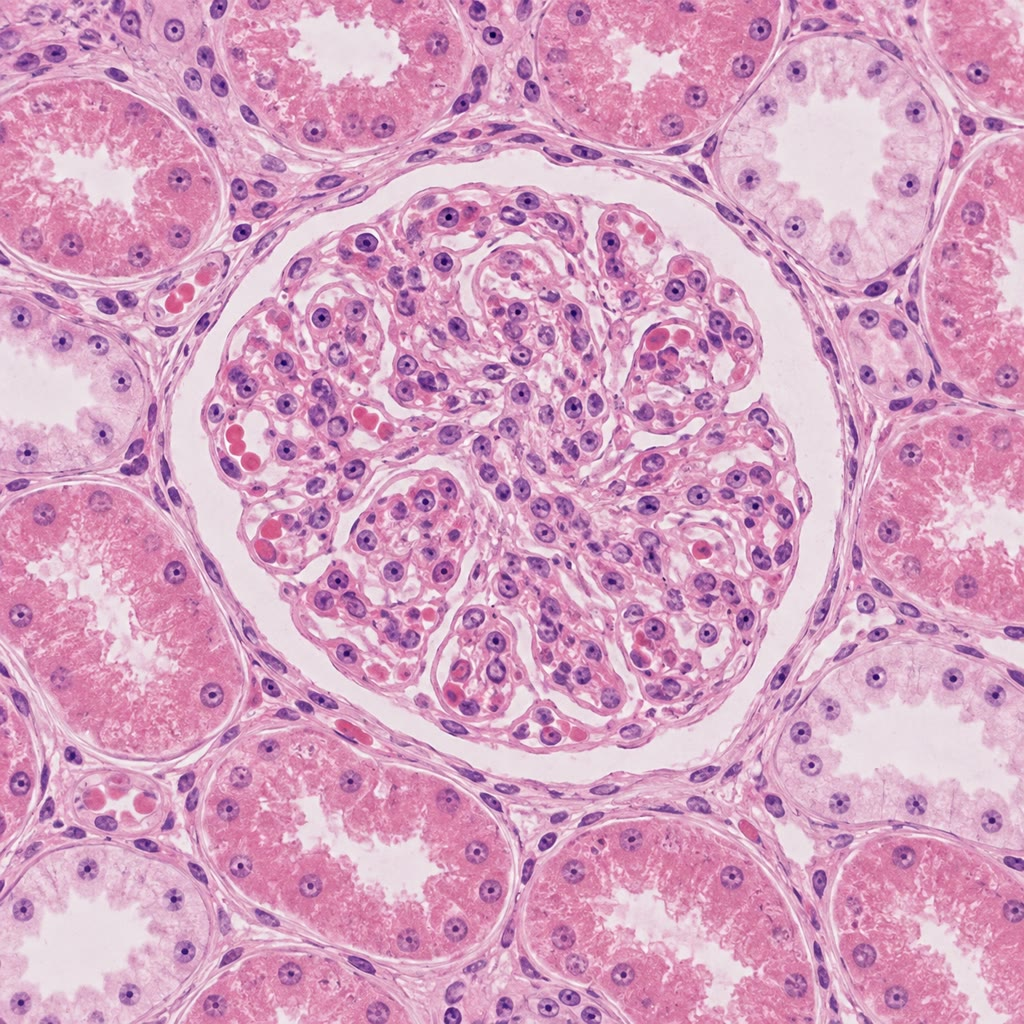
\includegraphics[width=0.46\linewidth]{images/book5/ai/b5-20-kidney-section.jpg}\hspace{0.04\linewidth}
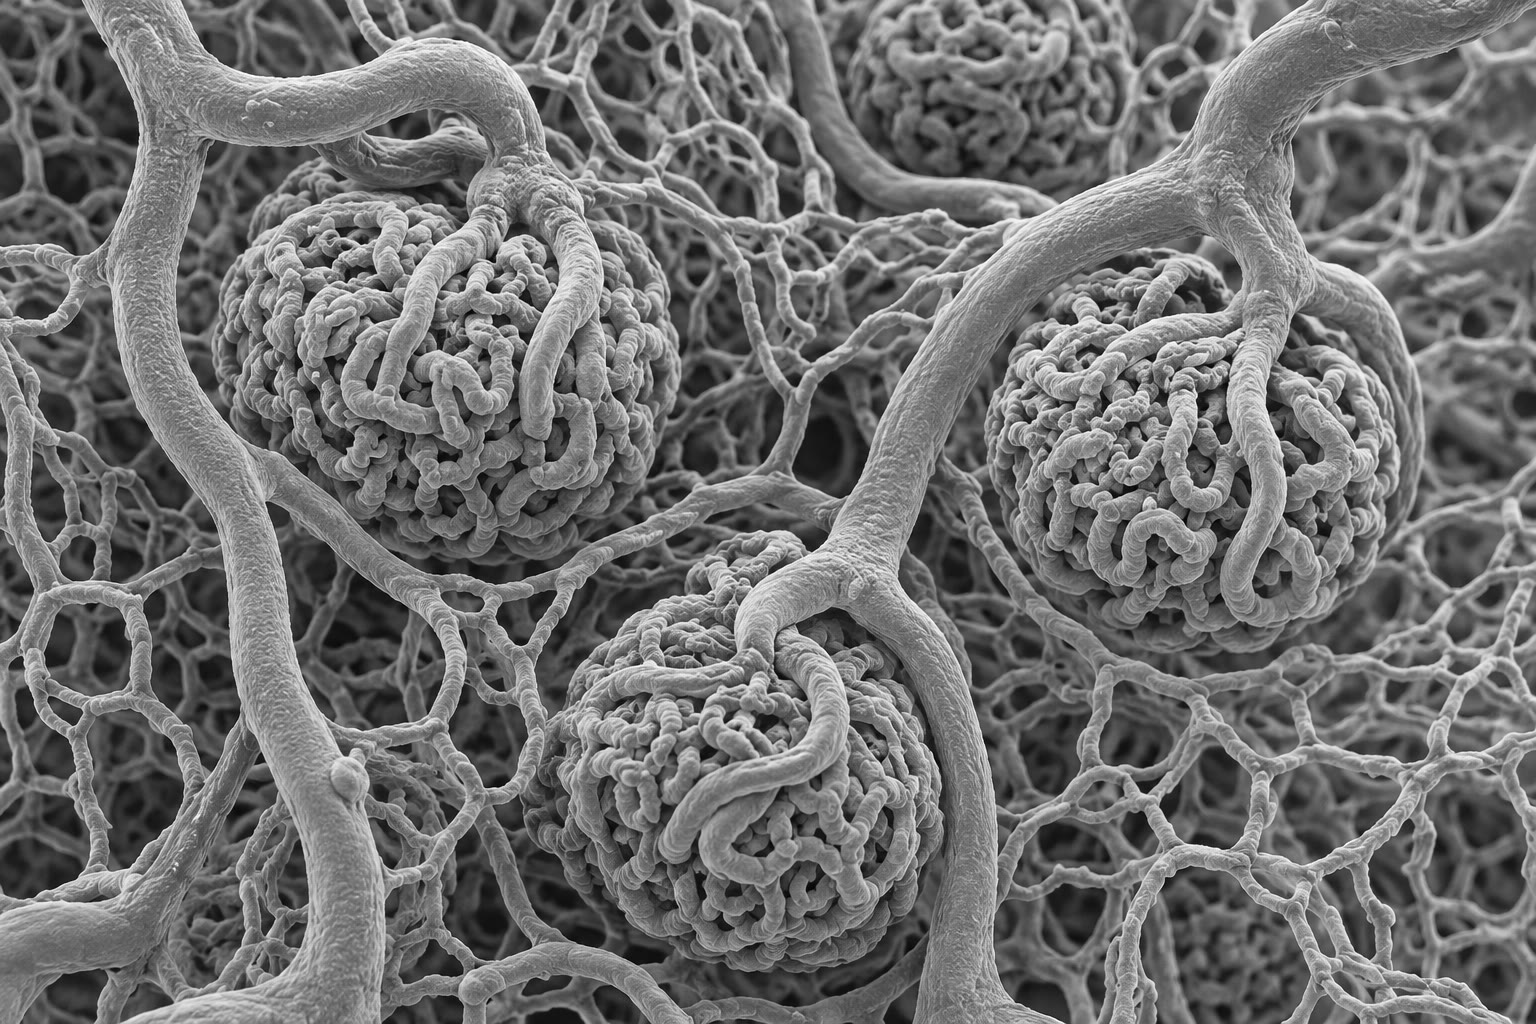
\includegraphics[width=0.46\linewidth]{images/book5/ai/b5-20-nephron-cast.jpg}

{\small Kiri: korteks ginjal dalam irisan --- sebuah \omterm{def:b3:renal-osmoregulation:nephron}{glomerulus} di dalam kapsulnya
di antara penampang \omterm{def:b3:renal-osmoregulation:nephron}{tubulus proksimal} dan distal. Kanan: sebuah cetakan
pembuluh korteksnya, tiap bola benangnya sebuah \omterm{def:b3:renal-osmoregulation:nephron}{glomerulus} dengan pembuluh aferen
dan eferennya di antara kapiler peritubulusnya.}
\end{omfigure}

\section{Hewan lain, penyelesaian lain}

\begin{definition}[Osmoregulasi di antara hewan]\label{def:b3:renal-osmoregulation:comparative}
\index{tubulus Malpighi}\index{kelenjar garam}\index{sel klorida}%
\index{air metabolisme}\index{ketebalan medula nisbi}
Ikan air tawar hidup di dalam sebuah medium sepersepuluh \omterm{def:b3:renal-osmoregulation:problem}{osmolaritas} darahnya:
airnya membanjir masuk lewat insangnya, garamnya bocor keluar, dan mereka mengekskresikan sebuah
kemih encer yang berlimpah lalu mengambil garam secara aktif lewat \emph{sel
klorida} insangnya, tanpa pernah minum. Teleostei laut, yang darahnya
sepertiga dari \omterm{def:b3:renal-osmoregulation:problem}{osmolaritas} lautnya, kehilangan air lewat insangnya lalu meminum
air laut, lalu memompa garamnya keluar lewat sel klorida yang sama yang dibalik,
sambil menjaga kemihnya tetap sedikit; hiu justru menjaga darahnya iso-osmotik
dengan lautnya dengan menahan urea (dan trimetilamina oksida untuk memantapkan
proteinnya terhadapnya), lalu mengekskresikan garam berlebih lewat sebuah kelenjar
rektum. Burung laut dan reptil laut mengusung \emph{kelenjar garam} di atas
matanya yang menyekresikan sebuah air garam dua kali seasin lautnya, yang membuat seekor
albatros dapat minum dari samuderanya. Serangga menapis lewat
\emph{tubulus Malpighi} yang digerakkan sekresi kalium aktif alih-alih
tekanan darah, lalu menyerap kembali air di dalam rektumnya sedemikian tuntasnya
sehingga kotoran seekor kumbang gurun kering. Di antara mamalia, daya
pemekatannya berskala dengan panjang lengkungnya relatif terhadap
ukuran ginjalnya (yakni \emph{ketebalan medula nisbi}): seekor berang-berang
sanggup \qty{500}{mOsm/L}, seorang manusia \num{1200}, seekor unta \num{3000},
tikus kanguru \num{5500} --- yang membuatnya dapat hidup dari \emph{air
metabolisme} yang dilepaskan ketika makanannya dioksidasi, sekitar \qty{0.6}{g} air
tiap gram pati, dengan sebuah hidung yang memulihkan air dari tiap
embusan napasnya.
\end{definition}

\begin{omfigure}
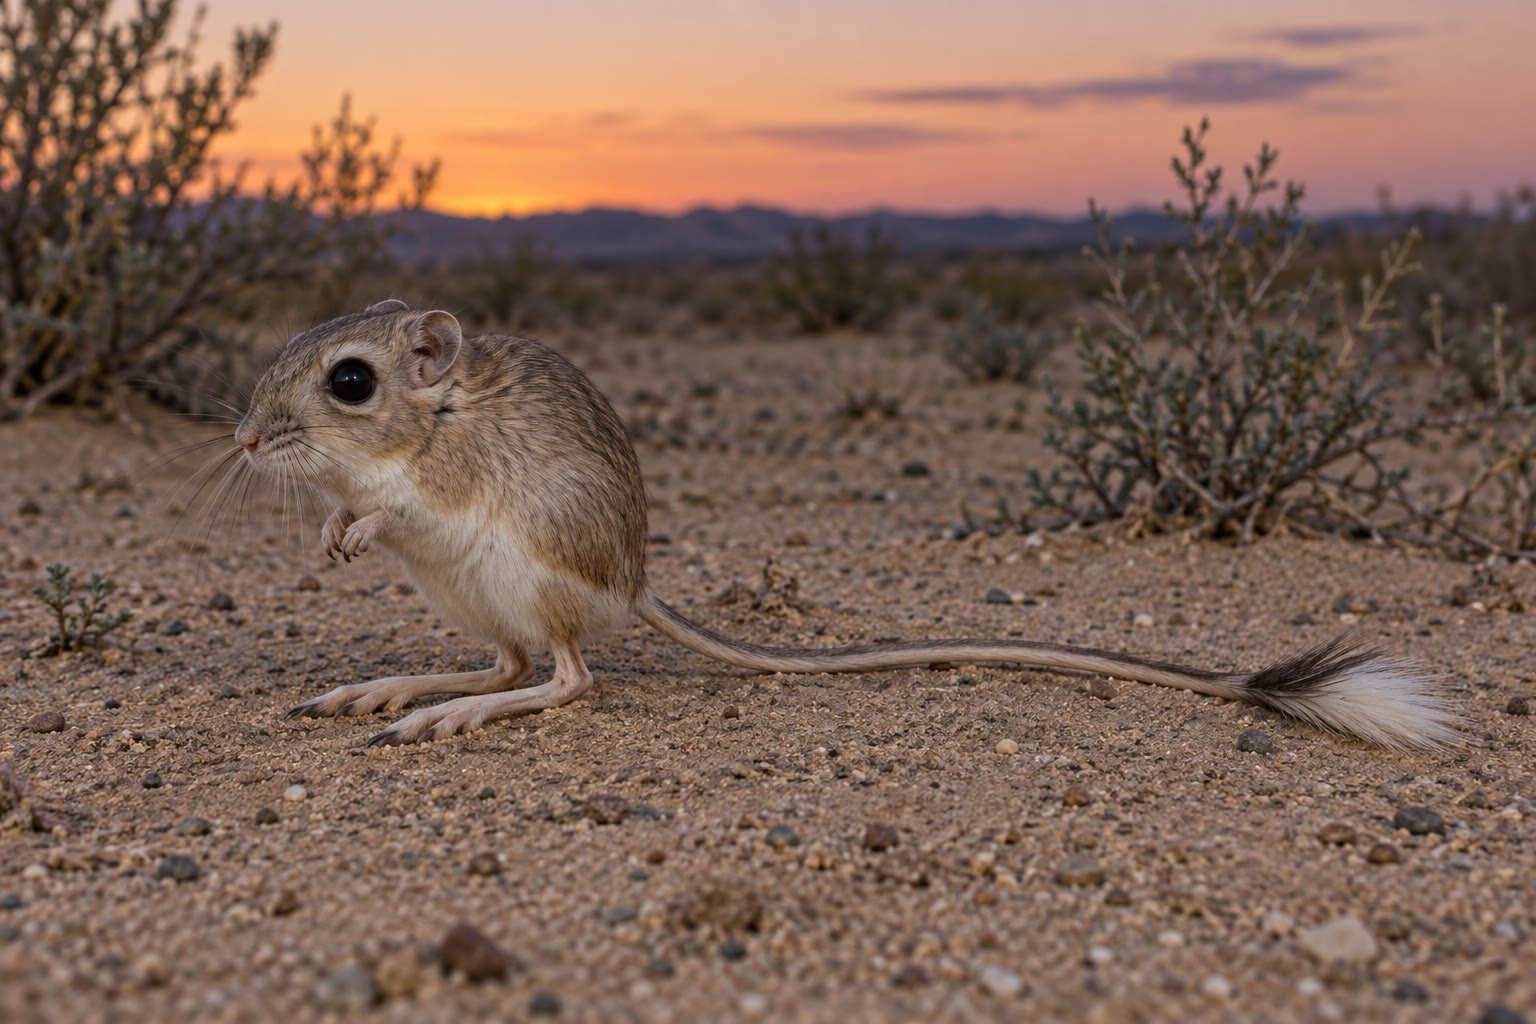
\includegraphics[width=0.56\linewidth]{images/book5/ai/b5-20-kangaroo-rat.jpg}

{\small Seekor tikus kanguru, yang tidak pernah minum: \omterm{def:b3:renal-osmoregulation:nephron}{lengkung Henle} yang panjang, sebuah kemih
lima kali sepekat air laut, sebuah hidung dingin yang mengembunkan
air tiap napasnya, dan sebuah makanan yang oksidasinya membuat semua air
yang diperlukannya.}
\end{omfigure}

\begin{remark}[Ginjal sebagai sebuah masalah rancangan]\label{rem:b3:renal-osmoregulation:design}
Ginjal mamalia menapis empat puluh kali volume plasmanya tiap hari hanya
untuk mengambil kembali nyaris semuanya: sebuah rancangan yang boros, yang maksudnya adalah
bahwa menapis semuanya lalu menyerap kembali secara terpilih lebih sederhana daripada
menyekresikan secara terpilih tiap limbah yang mungkin muncul. Ongkosnya adalah
\qty{7}{\%} metabolisme istirahat yang dibelanjakan memompa natrium kembali, dan
kerentanannya adalah tapisannya yang halus, yang gagal perlahan di bawah
tekanan tinggi dan glukosa tinggi. Kecerdikannya adalah lengkung arus
baliknya, yakni sebuah alat yang juga ditemukan di dalam gelembung renang ikan laut dalam, tungkai
burung perancah, dan hidung hewan pengerat gurun, yang dengannya sebuah selisih setempat
yang kecil dan terjangkau ditumpuk menjadi sebuah selisih yang besar --- yakni gagasan
yang sama, pada tiap hal, bahwa sebuah landaian dapat dibangun dari aliran.
\end{remark}

\section{Latihan}

\begin{exercise}[$\star$]\label{exo:b3:renal-osmoregulation:1}
Namailah ruas \omterm{def:b3:renal-osmoregulation:nephron}{nefron} itu berurutan lalu nyatakanlah satu hal yang dilakukan
masing-masing.
\end{exercise}

\begin{exercise}[$\star$]\label{exo:b3:renal-osmoregulation:2}
Definisikanlah bersihan. Sebuah zat berkepekatan plasma
\qty{2}{mg/mL}, berkepekatan kemih \qty{100}{mg/mL}, dan aliran kemihnya
\qty{1.5}{mL/min}. Hitunglah bersihannya lalu katakanlah apakah ia
diserap kembali, disekresikan, atau tidak keduanya, bila LFG-nya \qty{120}{mL/min}.
\end{exercise}

\begin{exercise}[$\star$]\label{exo:b3:renal-osmoregulation:3}
Mengapa seekor ikan air tawar tidak pernah minum dan seekor ikan laut minum
terus-menerus? Apa yang dilakukan insangnya pada masing-masing?
\end{exercise}

\begin{exercise}[$\star$]\label{exo:b3:renal-osmoregulation:4}
Apa \omterm{prop:b3:renal-osmoregulation:countercurrent}{efek tunggal} \omterm{def:b3:renal-osmoregulation:nephron}{lengkung Henle}, cabang mana yang menghasilkannya,
dan mengapa kedua cabangnya harus berbeda pada keterlewatan airnya?
\end{exercise}

\begin{exercise}[$\star\star$]\label{exo:b3:renal-osmoregulation:5}
Tekanan kapiler \omterm{def:b3:renal-osmoregulation:nephron}{glomerulus} \qty{60}{mmHg}, ruang Bowman
\qty{18}{mmHg}, tekanan onkotik plasma \qty{28}{mmHg} pada ujung
aferennya yang naik menjadi \qty{35}{mmHg} pada ujung eferennya. Hitunglah tekanan
penapisan neto pada tiap ujungnya lalu jelaskanlah mengapa penapisannya dapat berhenti
sebelum ujung kapilernya. Apa yang disiratkannya bagi pengaruh
aliran plasma pada LFG-nya?
\end{exercise}

\begin{exercise}[$\star\star$]\label{exo:b3:renal-osmoregulation:6}
Bersihan kreatinin seorang pasien \qty{40}{mL/min}. Natrium plasmanya
\qty{140}{mmol/L}, natrium kemihnya \qty{70}{mmol/L}, aliran kemihnya
\qty{1}{mL/min}. Hitunglah muatan natrium yang ditapis, ekskresinya,
bagian yang diserap kembali, dan bersihan natriumnya.
\end{exercise}

\begin{exercise}[$\star\star$]\label{exo:b3:renal-osmoregulation:7}
Seseorang memakan makanan yang menghasilkan \qty{900}{mOsm} zat terlarut tiap hari lalu dapat
memekatkan sampai \qty{1200}{mOsm/L}. Berapa volume kemih minimumnya? Bila penyakit
ginjal menurunkan maksimumnya ke \qty{400}{mOsm/L}, berapa banyak yang harus
diminumnya untuk tetap seimbang, dengan memperhitungkan \qty{0.9}{L} kehilangan tak terasa?
\end{exercise}

\begin{exercise}[$\star\star$]\label{exo:b3:renal-osmoregulation:8}
Ramalkanlah volume dan \omterm{def:b3:renal-osmoregulation:problem}{osmolaritas} kemihnya, natrium plasmanya, dan
keadaan hausnya pada (a) diabetes insipidus, (b) sekresi vasopresin yang
tidak pada tempatnya oleh sebuah \omterm{def:b3:cancer-biology:hallmarks}{tumor}, (c) kelebihan \omterm{def:b3:renal-osmoregulation:controls}{aldosteron}, (d) sebuah makanan tanpa
garam selama sepekan.
\end{exercise}

\begin{exercise}[$\star\star$]\label{exo:b3:renal-osmoregulation:9}
Hitunglah \omterm{prop:b3:renal-osmoregulation:water}{bersihan air bebas} bagi kemih \qty{100}{mOsm/L} pada
\qty{6}{mL/min} dan bagi kemih \qty{1000}{mOsm/L} pada
\qty{0.6}{mL/min}, dengan plasmanya pada \qty{300}{mOsm/L}. Tafsirkanlah masing-masing.
\end{exercise}

\begin{exercise}[$\star\star\star$]\label{exo:b3:renal-osmoregulation:10}
Modelkanlah lengkungnya sebagai $n$ tahap yang padanya cairan yang naik pada tiap
tahap \qty{200}{mOsm/L} di bawah interstisiumnya dan cairan yang turun
sama dengannya, dengan cairan yang masuk pada \qty{300}{mOsm/L}. Berhujahlah
bahwa \omterm{def:b3:renal-osmoregulation:problem}{osmolaritas} keadaan mantap di tikungannya dapat mendekati $300 +
200n$, sehingga landaiannya dibatasi panjang lengkungnya dan
\omterm{prop:b3:renal-osmoregulation:countercurrent}{efek tunggal} pompanya, lalu katakanlah apa yang menetapkan $n$ secara fisis.
\end{exercise}

\begin{exercise}[$\star\star\star$]\label{exo:b3:renal-osmoregulation:11}
Seekor tikus kanguru memakan \qty{5}{g} biji kering tiap hari, \qty{80}{\%} pati,
yang dioksidasi menjadi CO$_{2}$ dan air (\qty{0.6}{g} air tiap gram pati).
Ia harus mengekskresikan \qty{3}{mOsm} zat terlarut tiap hari pada \qty{5500}{mOsm/L},
lalu kehilangan \qty{1.5}{g} air tiap hari lewat penguapan dari sebuah hidung yang
memulihkan \qty{70}{\%} air di dalam napasnya. Imbangkanlah anggaran airnya lalu
katakanlah apakah ia bertahan hidup tanpa minum.
\end{exercise}

\begin{exercise}[$\star\star\star$]\label{exo:b3:renal-osmoregulation:12}
Dialisis melewatkan darah sepanjang satu sisi sebuah selaput dan dialisat sepanjang
sisi yang lain, dalam arus balik. Jelaskanlah mengapa aliran arus balik membersihkan
lebih banyak daripada aliran sejajar, taksirlah bersihan sebuah mesin yang
menyingkirkan urea dari \qty{300}{mL/min} darah dengan kemangkusan \qty{70}{\%},
lalu bandingkanlah dengan dua ginjal sepanjang sepekan bila mesinnya
berjalan empat jam tiga kali seminggu.
\end{exercise}

\section{Soal: Delapan Belas Ember Sehari}

\begin{problem}[{Soal akhir pekan --- tapisan sehari yang diikuti dari
glomerulusnya sampai kandung kemihnya: tekanan Starling, bersihan
empat zat, ambang glukosanya, anggaran airnya dari pengenceran maksimal
sampai air laut, serta neraca seekor hewan pengerat gurun, berakhir pada
LFG-nya, volume kemih wajibnya, dan air neto yang dihasilkan seliter air laut}]
\label{pb:b3:renal-osmoregulation:1}
Data: $K_{f} = \qty{12.5}{mL/min/mmHg}$; $P_{\text{KG}} = \qty{55}{mmHg}$,
$P_{\text{RB}} = \qty{15}{mmHg}$, $\pi_{\text{KG}} = \qty{30}{mmHg}$.
Plasma: inulin \qty{0.5}{mg/mL}, kreatinin \qty{0.01}{mg/mL}, urea
\qty{5}{mmol/L}, glukosa \qty{5}{mmol/L}, para-aminohipurat
\qty{0.02}{mg/mL}, Na$^{+}$ \qty{140}{mmol/L}, \omterm{def:b3:renal-osmoregulation:problem}{osmolaritas}
\qty{290}{mOsm/L}. Aliran kemih \qty{1}{mL/min}: inulin \qty{62.5}{mg/mL},
kreatinin \qty{1.3}{mg/mL}, urea \qty{250}{mmol/L}, glukosa $0$,
para-aminohipurat \qty{13}{mg/mL}, Na$^{+}$ \qty{100}{mmol/L},
\omterm{def:b3:renal-osmoregulation:problem}{osmolaritas} \qty{600}{mOsm/L}. Hematokrit $0.45$. Glukosa $T_{m} =
\qty{375}{mg/min}$ (\qty{2.1}{mmol/min}). Zat terlarut harian \qty{600}{mOsm};
$U_{\max} = \qty{1200}{mOsm/L}$, $U_{\min} = \qty{50}{mOsm/L}$;
kehilangan tak terasa \qty{0.9}{L/d}; air laut \qty{1000}{mOsm/L}.

\medskip
\noindent\textbf{Bagian I --- Tapisannya.}
\begin{enumerate}
  \item Hitunglah tekanan penapisan neto dan LFG-nya.
  \item Ubahlah LFG-nya menjadi liter tiap hari. Berapa kali volume plasmanya
        (\qty{3}{L}) ditapis?
  \item Hitunglah bersihan inulinnya lalu bandingkanlah dengan LFG-nya.
        Hitunglah bersihan kreatininnya; mengapa ia sedikit lebih besar?
  \item Hitunglah bersihan para-aminohipuratnya (yakni aliran plasma
        ginjalnya), aliran darah ginjalnya, dan pecahan penapisannya.
  \item Arteriol eferennya menyempit, yang menaikkan $P_{\text{KG}}$ ke
        \qty{60}{mmHg}. Berapa LFG barunya? Mengapa obat yang menghalangi angiotensin II
        menurunkan LFG-nya sedikit pada ginjal yang sehat lalu melindungi ginjal
        yang diabetes?
  \item Protein muncul di dalam kemihnya pada \qty{3}{g/d}. Lapisan mana dari
        tapisannya yang telah gagal, dan apa yang terjadi pada tekanan onkotik
        plasmanya dan pada jaringannya bila hal itu berlanjut?
\end{enumerate}

\medskip
\noindent\textbf{Bagian II --- Penanganannya.}
\begin{enumerate}[resume]
  \item Urea: muatan yang ditapis, ekskresinya, bagian yang diserap kembali, dan
        bersihannya.
  \item Natrium: muatan yang ditapis tiap hari dalam mol dan gram, ekskresinya,
        dan bagian yang diserap kembali. Berapa kilogram garam yang akan
        hilang dalam sehari bila tidak ada yang diserap kembali?
  \item Glukosa: muatan yang ditapis dalam mmol/min dan dalam gram tiap hari; adakah yang
        diekskresikan? Pada glukosa plasma berapa muatan yang ditapis mencapai
        $T_{m}$ (yakni ambangnya)?
  \item Seorang diabetes berglukosa plasma \qty{20}{mmol/L}. Berapa glukosa yang diekskresikan
        tiap menit dan tiap hari dalam gram, dan berapa volume kemih tambahannya bila
        tiap \qty{300}{mOsm} glukosa mengusung \qty{1}{L} pada
        kepekatan yang berlaku. Jelaskanlah rasa haus dan penurunan bobot
        diabetes yang tidak diobati.
  \item Menyerap kembali natrium berongkos satu ATP tiap tiga Na$^{+}$. Berapa
        mol ATP tiap hari yang dibelanjakan ginjalnya pada natrium, dan berapa
        kilojoule (\qty{50}{kJ/mol})? Bandingkanlah dengan
        \qty{7}{MJ/d} keadaan istirahat.
  \item Jelaskanlah mengapa ginjalnya menapis lalu menyerap kembali alih-alih
        menyekresikan tiap limbahnya, menurut apa yang harus dikenali
        tubulusnya.
\end{enumerate}

\medskip
\noindent\textbf{Bagian III --- Air.}
\begin{enumerate}[resume]
  \item Bersihan osmolar $U_{\text{osm}}V/P_{\text{osm}}$ dari
        datanya, dan \omterm{prop:b3:renal-osmoregulation:water}{bersihan air bebasnya}. Apakah orangnya menghemat atau
        membuang air?
  \item Volume kemih minimum bagi zat terlarut hariannya; maksimumnya (pada
        $U_{\min}$); kebutuhan air harian totalnya pada minimumnya, dengan
        kehilangan tak terasanya.
  \item Seliter air laut diminum. Berapa banyak kemih yang diperlukan untuk
        mengekskresikan garamnya pada $U_{\max}$, dan berapa perolehan air neto
        sebelum zat terlarut hari itu sendiri dihitung? Sesudahnya?
  \item Vasopresinnya tidak ada (diabetes insipidus) dan kemihnya tetap
        pada $U_{\min}$. Berapa volume kemih hariannya bagi zat terlarut yang sama, dan berapa
        air yang harus diminum tiap hari untuk menjaga keseimbangannya?
  \item Bir pada \qty{20}{mOsm/L}: berapa banyak yang dapat diminum tiap hari sebelum
        ginjalnya, pada $U_{\min}$, tidak lagi dapat mengekskresikan airnya?
        (Air yang berlebih dari yang dapat diusung zat terlarutnya pada $U_{\min}$
        menimbun.)
  \item Sesudah semalam tanpa air, \omterm{def:b3:renal-osmoregulation:problem}{osmolaritas} plasmanya
        \qty{298}{mOsm/L}. Naik berapa persen ia, dan apa yang dilakukan
        hipotalamusnya? Taksirlah kekurangan airnya bila air tubuh
        totalnya \qty{42}{L} dan zat terlarutnya tidak berubah.
  \item Jelaskanlah mengapa seorang pelari maraton yang meminum \qty{6}{L} air
        sambil mengeluarkan keringat bergaram dapat mengalami natrium plasma yang rendah berbahaya,
        dan apa yang harus dilakukan ginjalnya untuk mencegahnya.
\end{enumerate}

\medskip
\noindent\textbf{Bagian IV --- Gurunnya.}
\begin{enumerate}[resume]
  \item Seekor tikus kanguru mengekskresikan \qty{3}{mOsm} tiap hari pada \qty{5500}{mOsm/L}.
        Berapa volume kemihnya? Bandingkanlah dengan volume yang akan diperlukan
        sebuah ginjal manusia bagi zat terlarut yang sama pada maksimumnya sendiri.
  \item Makanannya menghasilkan \qty{2.4}{g} \omterm{def:b3:renal-osmoregulation:comparative}{air metabolisme} tiap hari dan ia
        kehilangan \qty{1.6}{g} lewat napas dan \qty{0.3}{g} di dalam tinja.
        Imbangkanlah anggarannya dengan kemih pertanyaan 20.
  \item Seekor unta memekatkan sampai \qty{3000}{mOsm/L} lalu tahan kehilangan
        \qty{25}{\%} air tubuhnya. Bagi seekor unta \qty{500}{kg} dengan
        \qty{65}{\%} air, berapa banyak yang dapat hilang, dan berapa hari yang
        ditutupinya pada kehilangan \qty{5}{L/d}?
  \item Seekor burung laut memakan \qty{200}{g} ikan lalu meminum \qty{100}{mL}
        air laut tiap hari, yang memasukkan \qty{150}{mmol} NaCl. \omterm{def:b3:renal-osmoregulation:comparative}{Kelenjar garamnya}
        menyekresikan pada \qty{800}{mmol/L}. Berapa banyak air garam yang
        dihasilkannya, dan mengapa kelenjarnya lebih baik daripada ginjalnya (yang pada
        burung memekatkan hanya sampai \qty{600}{mOsm/L}) untuk hal ini?
  \item Seekor ikan air tawar \qty{100}{g} memperoleh \qty{30}{\%} massa tubuhnya
        berupa air tiap hari lewat insangnya. Berapa banyak kemih yang harus
        dibuatnya, pada \omterm{def:b3:renal-osmoregulation:problem}{osmolaritas} berapa relatif terhadap darahnya, dan apa yang akan
        terjadi pada garamnya tanpa pengambilan aktif?
  \item Ringkaslah: LFG-nya (pertanyaan~1), volume kemih wajibnya
        (pertanyaan~14), dan air neto dari seliter air laut sesudah
        zat terlarut hari itu dihitung (pertanyaan~15).
\end{enumerate}
\end{problem}
